\documentclass[12pt]{article}
\usepackage[T1]{fontenc}
\usepackage[utf8]{inputenc}
\usepackage{url}
\usepackage{enumerate}
\usepackage[top=3cm, bottom=3cm]{geometry}
\usepackage{graphicx} 
\usepackage{enumitem}
\usepackage{natbib}
\usepackage{listings}
\usepackage{float}
\bibpunct{[}{]}{,}{a}{}{;}
\setcitestyle{super}

% Variables
\newcommand{\assignmentname}{Assignment 1}
\newcommand{\coursename}{Statistical Methods in Machine Learning}
\newcommand{\studentnameOne}{Bjarki Madsen (lch929)}
\newcommand{\studentnameTwo}{Disha Singh (cfn492)}
\newcommand{\studentnameThree}{Sokratis Siozos - Drosos (dnb823)}
\newcommand{\department}{Department of Computer Science}
\newcommand{\institution}{Copenhagen University}
\newcommand{\location}{Copenhagen, Denmark}

\begin{document}

\renewcommand\refname{References}

\title{\assignmentname \\ {\Large {\textsc \coursename}}}
\author{
        \studentnameOne \\
        \studentnameTwo \\
        \studentnameThree \\ \\
                \department \\
        \institution \\
        \location
}
\date{\today}

\maketitle
\thispagestyle{empty}

\pagebreak

\subsection*{I.2.1 Univariate Gaussian distributions}

  Figure \ref{fig:gaussian_distribution} shows plot of three different parameters. The bell shaped curve for  each of the plot has different peak as shown using the Gaussian formula. 

  \begin{figure}[h]
    \centering
        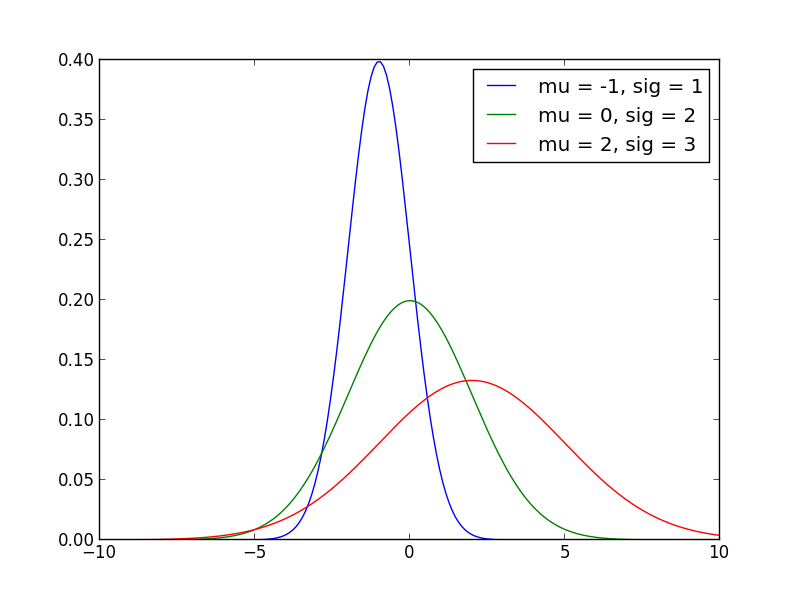
\includegraphics[width=1.0\textwidth]{figures/figure_I_2_1}
    \caption{Gaussian distribution with different $\mu$ and $\sigma$.}
    \label{fig:gaussian_distribution}
  \end{figure}

\subsection*{I.2.2 Sampling from a multivariate Gaussian distribution}
  
 Figure \ref{fig:multivariate_gaussian_distribution} shows plot of the dataset as a result using python code implementation.
 
  \begin{figure}[H]
    \centering
        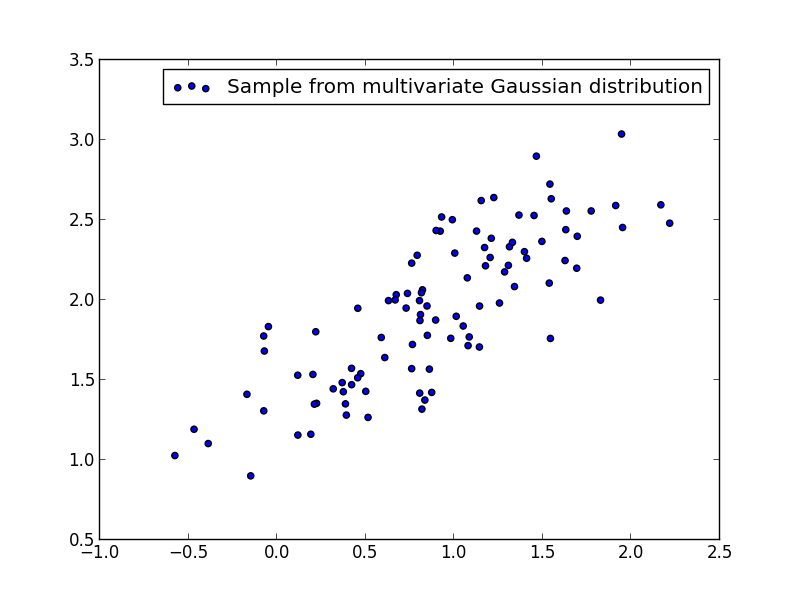
\includegraphics[width=1.0\textwidth]{figures/figure_I_2_2}
    \caption{Samples from multivariate Gaussian distribution.}
    \label{fig:multivariate_gaussian_distribution}
  \end{figure}
  
\subsection*{I.2.3 Means}
  
  Figure \ref{fig:distribution_with_means} shows plot of the data with two means in green and red color. We calculated the mean of the dataset and plotted it on top of the sampled data together with the actual mean. The means tend to deviate as the Maximum Likelihood Estimator will choose the mean that maximizes the probability of occurrence of given data points and when we consider a part of the distribution their can be a deviation from distribution mean.  

  \begin{figure}[H]
    \centering
        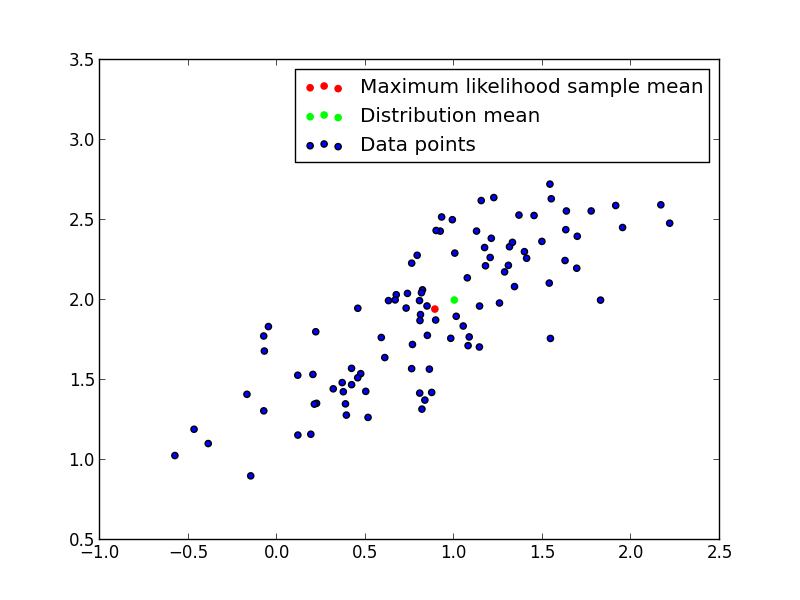
\includegraphics[width=1.0\textwidth]{figures/figure_I_2_3}
    \caption{Plot of the data with two means in green and red color.}
    \label{fig:distribution_with_means}
  \end{figure}

\subsection*{I.2.4 Covariance: The geometry of multivariate Gaussian distributions}

  Figure \ref{fig:distribution_with_eigenvectors} shows the plot of the datasets. Length of the scaled and rotated eigenvectors represents the spread from the sample mean in orthogonal directions. The eigenvector with the highest eigenvalue is the direction along which the data has the maximum variance. 

  \begin{figure}[H]
    \centering
        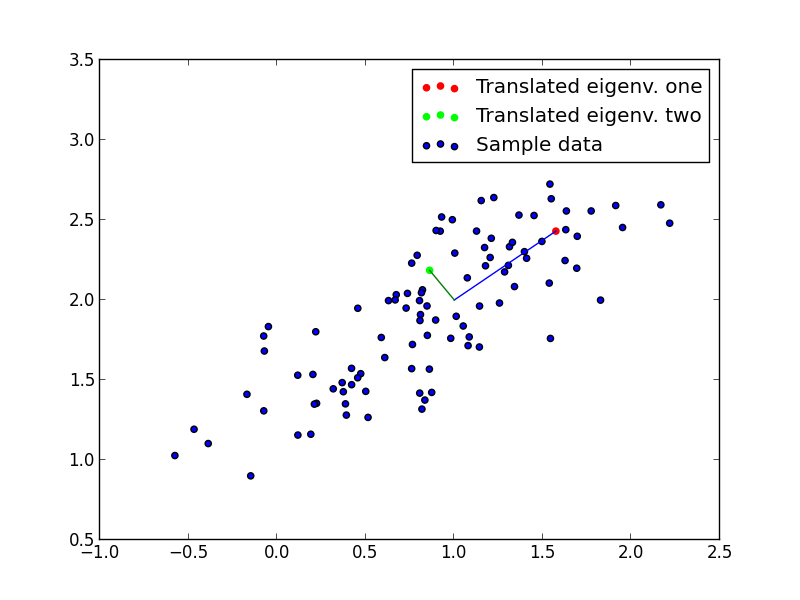
\includegraphics[width=1.0\textwidth]{figures/figure_I_2_4}
    \caption{Dataset with eigenvectors scaled and translated are orthogonal}
    \label{fig:distribution_with_eigenvectors}
  \end{figure}

  \begin{figure}[H]
    \centering
        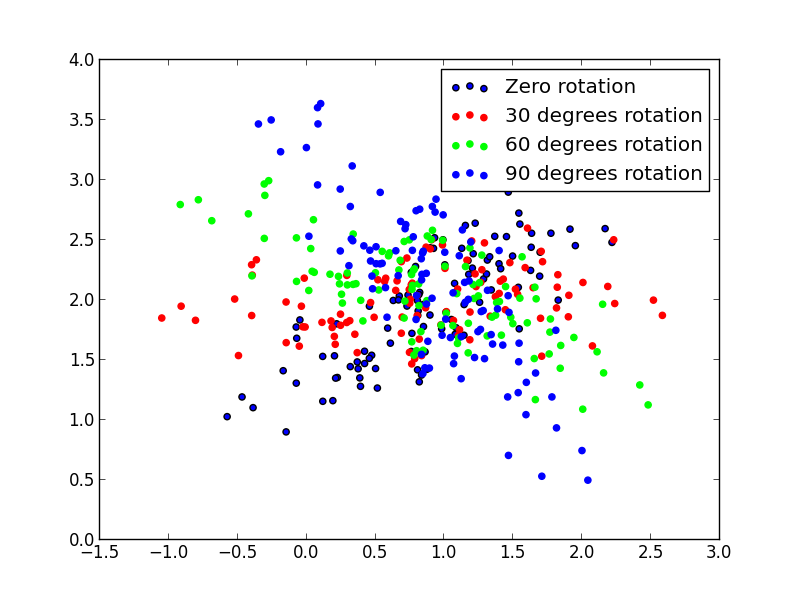
\includegraphics[width=1.0\textwidth]{figures/figure_I_2_4_rot}
    \caption{Combined plot of rotated dataset }
    \label{fig:distribution_rotated}
  \end{figure}

\section*{I.3 Classification}

\subsection*{I.3.1 Nearest neighbor}

   We used the most simple and naive way to determine the nearest neighbors: for a given point in $S_{test}$, calculate the distances, $D$, to every point in $S_{train}$ and store it in a map. When each $d \in D$ has been calculated, sort $D$ in ascending order and take the first $k$ neighbors, resulting in the $k$ nearest neighbors. 

   The Nearest Neighbor algorithm was performed for $k = 1,3,5$. As described by the project the \textit{IrisTrain2014.dt} file was used as the train data and then the \textit{IrisTest2014.dt} as test data. Furthermore, \textit{IrisTrain2014.dt} file was used for both training and testing. The results about the accuracy are reported in table \ref{table:accuracy_nearest_neigbor}.

  \begin{table}[h]
    \centering
    \begin{tabular}{| c | c | c |}
      \hline
        $k$ & Training only & With test \\
      \hline
        1 & 1.000 & 0.816 \\
        3 & 0.860 & 0.789 \\
        5 & 0.830 & 0.684 \\
      \hline
    \end{tabular}
    \caption{Accuracy for $k$ nearest neighbor classifier}
    \label{table:accuracy_nearest_neigbor}
  \end{table}

  As expected, the results show 100\% accuracy for $k = 1$ when considering the training set only. It can also be observed that using the same data for training and testing results in significantly higher accuracy scores than using different data for training and testing. 

  The code for this section is in the function called \texttt{i\_3\_2()}.

\subsection*{I.3.2 Hyperparameter selection using cross-validation}

  We performed a 5-fold cross-validation on the \textit{IrisTrain2014.dt} training data to determine what value of $k$ is best for maximum accuracy. We divided the data into 5 parts and for each iteration we used one part for training, $S_{train}$ and the other 4 for testing, $S_{test}$. Each iteration also took the mean accuracy of calculating $k$ nearest neighbors for $k = 1, 3, 5, \dots, 25$. The results of the mean accuracy is shown in table \ref{table:mean_accuracy_cross_fold}.

  \begin{table}[h]
    \centering
    \begin{tabular}{| c | c |}
      \hline
        No. NN & Mean Accuracy \\
      \hline
        1 & 0.780 \\
        \textbf{3} & \textbf{0.800} \\
        5 & 0.750 \\
        7 & 0.770 \\
        9 & 0.780 \\
        11 & 0.780 \\
        13 & 0.780 \\
        15 & 0.780 \\
        17 & 0.780 \\
        19 & 0.780 \\
        21 & 0.780 \\
        23 & 0.770 \\
        25 & 0.760 \\
      \hline
    \end{tabular}
    \caption{Results using cross-validation showing $k_{best} = 3$}
    \label{table:mean_accuracy_cross_fold}
  \end{table}

  As it can be observed from the table, the best accuracy was achieved for $k = 3$. Performing the knn algorithm with $k = 3$ the accuracy on the test data is $0.789$, which is almost the same with the mean accuracy we got from the cross-validation.

  The code for this section is in the function called \texttt{i\_$3$\_$2$()}.

\subsection*{I.3.3 Data normalization}

  We computed the mean and the variance for each feature of the training data (lengths and widths), which was then used to normalize the unseen test data by using the following formula: 
  $$ X' = \frac{X - \mu}{\sigma}$$
  where $\mu$ and $\sigma$ is the mean and the standard deviation, respectively, for the corresponding feature, $X$. The mean and the variance for the training set and the normalized data set is shown in table \ref{table:mean_var_train_norm}. 

  We then performed 5-fold cross-validation on the normalized training data to find the hyperparameter $k$. The $k_{best}$ suggested by the cross-validation is $k = 1$ which gave 86\% accuracy, as seen in table \ref{table:norm-cross-validation}. The corresponding training and test errors given by the $k_{best}$ is shown in table \ref{table:error_train_test_norm}.

  \begin{table}[h]
    \centering
    \begin{tabular}{| c | c | c | c | c |}
      \hline
        set & $\mu$ length & $\sigma$ length & $\mu$ width & $\sigma$ width \\
      \hline
        train           & 5.756 & 0.689 & 0.302 & 0.002 \\
        test normalized & 0.208 & 1.073 & 0.432 & 1.252 \\
      \hline
    \end{tabular}
    \caption{Mean and variance for the features in the training set and normalized data set.}
    \label{table:mean_var_train_norm}
  \end{table}

  \begin{table}[h]
    \centering
    \begin{tabular}{| c | c |}
      \hline
        No. NN & Mean Accuracy \\
      \hline
        \textbf{1} &  \textbf{0.860} \\
        3 &  0.820 \\
        5 &  0.820 \\
        7 &  0.810 \\
        9 &  0.840 \\
        11 & 0.850  \\
        13 & 0.840  \\
        15 & 0.800  \\
        17 & 0.800  \\
        19 & 0.820  \\
        21 & 0.810  \\
        23 & 0.810  \\
        25 & 0.810  \\
      \hline
    \end{tabular}
    \caption{Results using cross-validation on normalized training data showing $k_{best} = 1$}
    \label{table:norm-cross-validation}
  \end{table}

  \begin{table}[h]
    \centering
    \begin{tabular}{| c | c | c |}
      \hline
        $k_{best}$ & Training & Test \\
      \hline
        1 & 0.0 & 0.211 \\
      \hline
    \end{tabular}
    \caption{Training and test error considering normalized data.}
    \label{table:error_train_test_norm}
  \end{table}

\end{document}
% End of document.







